\documentclass[12pt]{article}

\usepackage{algorithmic}
\usepackage{amsmath}
\usepackage{graphicx}
\usepackage{hyperref}
\usepackage{booktabs}

\begin{document}

\title{CSI709 Midterm \\
Problem 2}
\author{
        Geoffrey Ulman \\
        George Mason University\\
}
\date{\today}

\maketitle

\section{Results}

There are two classes of boats in the input image in Figure \ref{boats}: those with shiny white hulls, and those with light green canopies. My general approach was to build and combine two separate masks which detected ships of one type.

\begin{figure}
\centering
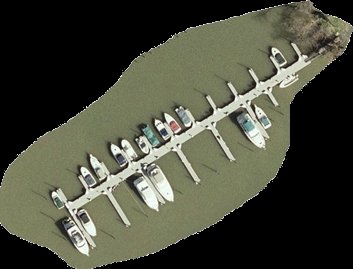
\includegraphics[width=0.30\textwidth]{boatsmall.jpg}
\caption{Input Image}
\label{boats}
\end{figure}

The shiny white hull mask used a cutoff in the lightness component of the image in the LUV colorspace. Pixels with a lightness of greater than \(15200\) were selected by the mask. This mask was combined with another simple cutoff mask on the LUV lightness component which masked off the area of interest (shown in Figure \ref{bordermask}). The intersection of the two masks is shown in Figure \ref{maskshiny}. This leaves a number of small light spots, mostly along the pier. It also creates multiple disconnected blobs on some ships where the sun reflect off the white hull at multiple points or where the dark canopy conceals the hull. If uncorrected, this could cause such ships to be counted multiple times. To remove the small glints from the pier and other non-ship areas of the image, areas smaller than 14 pixels were removed from the mask. The result of this operation is shown in Figure \ref{maskshinyminusblobs}.

\begin{figure}
\centering
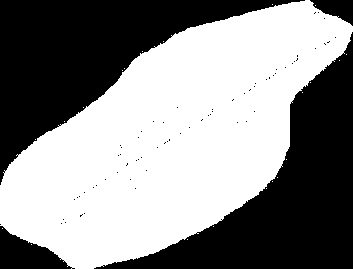
\includegraphics[width=0.30\textwidth]{border_mask.png}
\caption{Area of Interest Mask}
\label{bordermask}
\end{figure}

\begin{figure}
\centering
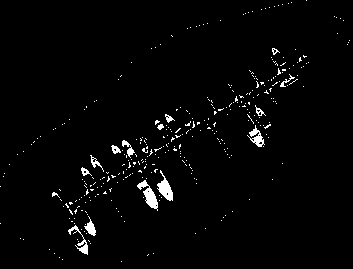
\includegraphics[width=0.30\textwidth]{mask_shiny.png}
\caption{Lightness Cutoff Mask}
\label{maskshiny}
\end{figure}

\begin{figure}
\centering
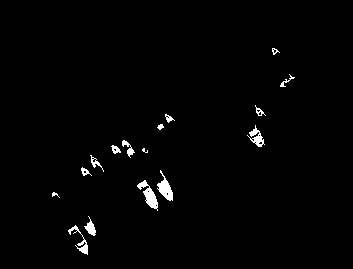
\includegraphics[width=0.30\textwidth]{mask_shiny_minus_blobs.png}
\caption{Lightness Cutoff Mask With Small Blobs Removed}
\label{maskshinyminusblobs}
\end{figure}

\begin{figure}
\centering
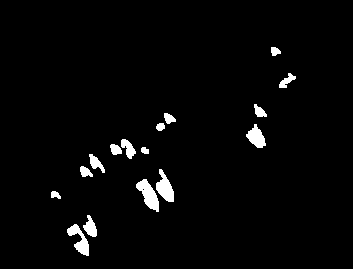
\includegraphics[width=0.30\textwidth]{mask_shiny_minus_blobs_blurred.png}
\caption{Blurred Lightness Cutoff Mask}
\label{maskshinyminusblobsblurred}
\end{figure}

To ensure that there is only one connected blob per ship, a convolution with a blur kernel (which emphasized the center pixel) was applied to the image. A cutoff was then applied to return to a 0/1 mask. The result of this operation is shown in Figure \ref{maskshinyminusblobsblurred}.

The above technique does not catch all ships because some are covered in light green canopies. To count these ships, another mask was used. This mask used a cutoff in the \(u\) component of the image in LUV colorspace. Pixels with a \(u\) value of less than \(-300\) or greater than \(-4000\) were selected by the mask. The result is shown in Figure \ref{maskgreencanopy}. This mask was then intersected with the area of interest mask from Figure \ref{bordermask} to remove the junk around the edges, before being unioned with the final shiny area mask from Figure \ref{maskshinyminusblobsblurred}. The result of the union is shown in Figure \ref{maskalmostfinal}.

\begin{figure}
\centering
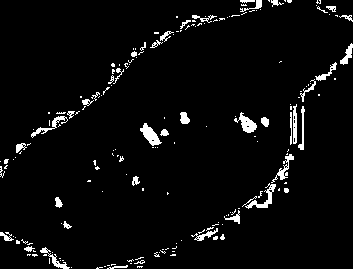
\includegraphics[width=0.30\textwidth]{mask_green_canopy.png}
\caption{Green Canopy Cutoff Mask}
\label{maskgreencanopy}
\end{figure}

\begin{figure}
\centering
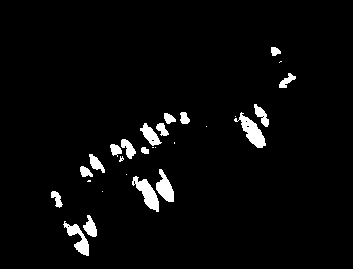
\includegraphics[width=0.30\textwidth]{mask_almost_final.png}
\caption{Final Mask}
\label{maskalmostfinal}
\end{figure}

Ships were then defined as contiguous sections of the final mask with more than 20 pixels. Figure \ref{finalcolor} highlights each such region in a random unique color. Figure \ref{finalmask} shows the portions of the initial image (see Figure \ref{boats}) that were selected by the mask (in order to verify that there are boats under those portions of the image). It should be noted that the algorithm does not attempt to define the entire outline of the boat, just to pick one spatially separated and distinct feature from each boat so that the number of boats can be calculated. It can be seen from these images that all 18 boats were detected.

\begin{figure}
\centering
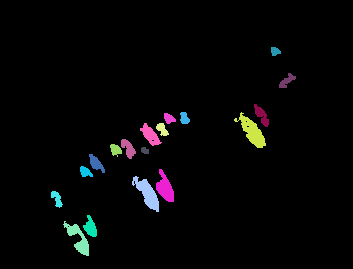
\includegraphics[width=0.30\textwidth]{final_color.png}
\caption{Detected Ships Shown In Unique Colors}
\label{finalcolor}
\end{figure}

\begin{figure}
\centering
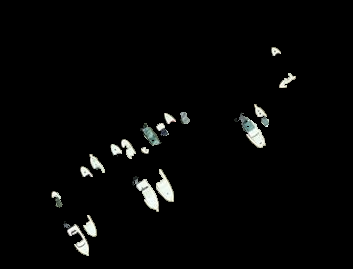
\includegraphics[width=0.30\textwidth]{final_mask.png}
\caption{Initial Image Masked Using Detected Ships }
\label{finalmask}
\end{figure}

\end{document}
